\chapter{RIOT-OS and The GNRC Network Stack}
\section{RIOT Operating System}
  RIOT, the friendly operating system for the Internet of Things, is a real-time operating system,
  specifically designed for low-end IoT devices with a minimal memory in order of $\approx$ 10K Byte
  \cite{riot}. It can run on devices with neither memory management unit (MMU) nor memory protection unit (MPU).

  Under the distribution of LGPLv2.1 License, RIOT is free and open-source software, meaning it can
  be used and distributed by anyone. Furthermore, this license allows the linkage of RIOT with
  proprietary software and supports the ability to be customized by the end users.

  The design objectives of RIOT focus on several key areas: optimizing resource usage such as RAM, 
  ROM, and power consumption; supporting a broad spectrum of configurations, from 8-bit to 32-bit MCUs, 
  and accommodating various boards and use cases; reducing code duplication across different setups; 
  ensuring most of the code is portable across supported hardware; offering user-friendly software 
  platform; and enabling real-time capabilities. To realize these goals, one of the principles that
  the RIOT follows is modularity. 

  RIOT is organized into software modules that are combined at compile time, centered around a kernel 
  offering minimal functionality. This modular approach allows the system to be built in a way that includes 
  only the necessary modules for a given use case. As a result, both memory usage and system complexity 
  are kept to a minimum in practical deployments. The code structure of RIOT is illustrated in
  Figure \ref{fig:riot_code}:
  
  \begin{itemize}
    \item \textbf{core} provides the kernels and basic data structures like linked lists, LIFOs,
    and ringbuffers.
    \item Four parts of hardware abstractions:
      \begin{enumerate}
        \item \textbf{cpu} implements functionalities of microcontroller.
        \item \textbf{boards} selects, maps and configures the used CPU and drivers.
        \item \textbf{drivers} implement the device drivers.
        \item \textbf{periph} provides unified access to microcontroller peripherals and is used by
        device drivers.
      \end{enumerate}
    \item \textbf{sys} implements libraries beyond kernel features, such as cryptography, networking, and file
    system.
    \item \textbf{pkg} contains third-party libraries which do not exist within the main code 
    repository.
  \end{itemize}

  \begin{figure}[h]
    \centering
    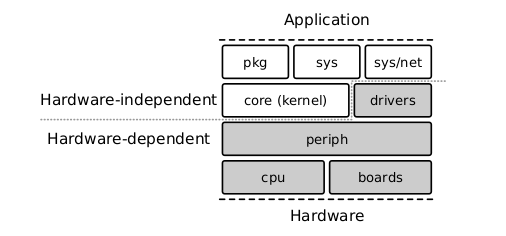
\includegraphics[width=0.8\linewidth]{riot_code}
    \caption{Structure elements of RIOT, see \cite[p.~3]{riot}}
    \label{fig:riot_code}
  \end{figure}

    Multi-threading is a builtin feature for RIOT to offer several benefits: (a) clear 
    logical separation between different tasks, (b) straightforward task prioritization, 
    and (c) easier integration of external code \cite[p.~4]{riot}. Various synchronization primitives, such
    as mutex, semaphore, and message passing (\textbf{msg}) are provided by RIOT kernel.
    Multi-threading can also be optional in the case of extremely low-memory usage of the application.

    RIOT's kernel employs a scheduler that uses fixed priorities and preemption with O(1) operations, 
    enabling soft real-time capabilities. Specifically, the time required to interrupt and switch 
    between threads is bounded by a small upper limit, as operations like context saving, selecting 
    the next thread, and context restoring are deterministic. The system follows a class-based 
    run-to-completion scheduling policy, where the highest-priority active thread is executed and 
    can only be interrupted by interrupt service routines (ISRs). This scheduler allows RIOT to 
    effectively prioritize tasks, ensuring that high-priority events can preempt lower-priority 
    tasks as needed.

    RIOT's scheduler operates in a tickless manner, meaning it does not rely on CPU time slices 
    or periodic system timer ticks. As a result, the system remains in a low-power state unless 
    an actual event occurs, such as an interrupt triggered by hardware. Wake-up events can be 
    initiated by a transceiver receiving a packet, timers expiring, buttons being pressed, or 
    similar activities. When no threads are in a running state and no interrupts are pending, 
    the system automatically switches to the idle thread, which has the lowest priority. 
    The idle thread, in turn, transitions the system into the most energy-efficient mode available 
    thereby reducing energy consumption.
\section{GNRC}
\subsection{Overview}
  - Design of the network stack
    
    - Northbound API with sock for application

    - Southbound API for network interface

  - Each network stack runs on its stack, communicate with each other through IPC api.
\subsection{The Packet Buffer - pktbuf}
  - The copy on write nature
  
  - Central packet buffer to reduce packet copy.
\subsection{GNRC's Module Registry - netreg}
  - What it is?
\subsection{A Common Inter-Modular API - netapi}
  - Does it still exist?
\subsection{Network Interfaces and Device Drivers}
  - Netif and how it works

